\documentclass[a4paper]{article}

\usepackage[english]{babel}  % Language support

%% Misc packages
\usepackage{framed}  % Enables frames around quote env.
\usepackage[hyphens]{url}
\usepackage{hyperref}  % \url command, properly working

%% Font selection
\usepackage{newpxtext,newpxmath}
\usepackage[T1]{fontenc}
\usepackage{microtype}

%% Listings (see https://www.ctan.org/pkg/minted for installation)
\usepackage[outputdir=.texpadtmp]{minted}
\setminted{	python3 = true,
			fontsize = \small, 
			frame = leftline, 
			framesep = 2\fboxsep}
\usepackage{upquote}  % TT quotes in listings

%% Graphics
\usepackage{graphicx, epstopdf}  % Support EPS figures
\epstopdfsetup{outdir=.texpadtmp/}

%% Bibliography
\usepackage[style=ieee, isbn=false]{biblatex}
\addbibresource{bibliography.bib}

%% Shortcuts
\usepackage{xspace}
\newcommand{\matlab}{\textsc{Matlab}\xspace}
\newcommand{\csv}{\texttt{CSV}\xspace}
\newcommand{\newpaper}[2]{\subsection*{\cite{#1}. \citetitle{#1}}

\begin{framed}\begin{quote}\begin{description}
	\item [Authors]\citeauthor{#1}
	\item [Title]\citetitle{#1}
	\item [Year]\citedate{#1}
	\item [Keywords]\texttt{#2}
\end{description}\end{quote}\end{framed}

}

%% Last package to be loaded (for compatibility issues)
\usepackage{cleveref}  % Allows en­hanced cross-ref­er­enc­ing fea­tures

%% Document details
\title{Piecewise analysis of stock market data}
\author{Paolo Antonini \and Davide Azzalini \and Fabio Azzalini}
\date{}

\usepackage{lipsum}  %TODO REV Remove

%% DOCUMENT
\begin{document}

\maketitle

\begin{abstract}
Time series data is characterised as large in size, high dimensionality and continuous updates. Moreover, it is always considered as a whole, instead of individual numerical fields. As a consequence, in order to analyse and mine time series data, segmentation and dimensionality reduction are essential, as well as trend identification. In particular, in the following pages we are going to collect and summarise some segmentation methods, applied in particular to stock market data. As a matter of fact, stock time series have their own characteristics over other time series. 
\end{abstract}




\section{Introduction}
The tasks of segmentation and dimensionality reduction, as well as identification of trends, are fundamental to allow a number of time series analysis and mining tasks. As a matter of fact, the fields of application of such procedures are numerous (ECG, exchange rates, sensors detections of any kind, \dots); moreover methods to perform this kind of preprocessing differ greatly, due to the nature and inherent characteristics of data. As a consequence, literature regarding these issues is vast. 

In particular, our focus in this report is on stock market data, which is outstandingly large in size, noisy and continuously updated. This paper is structured as follows: in \cref{sec:theory} we are providing a theoretical introduction and overview on the problem. Then in \cref{sec:methods} a number of research papers about dimensionality reduction and piecewise segmentation are listed and summarised. Then, in \cref{sec:implementations} we are going to present the implementations of a few methods. 



\section{Time series dimensionality reduction}\label{sec:theory}

In relevant literature, many algorithms have been proposed for representing time series into their segmented forms (i.e., dimensionally reduced), and many methods for creating time series representations can be found.

Generally, basic classification of algorithmic methods for segmentation implies their division into two great categories: offline, and online algorithms. The essence of offline segmentation is contained in the scanning and division of the entire time series $ T = \left\{ \left( y_1, t_1\right), \left(y_2, t_2 \right), \dots ,\left(y_n, t_n\right)\right\} $ into a number of segments, while the available number of data (data points) remains unchanged. On the other hand, in the online segmentation the uploading of new data points is performed in parallel with the execution of the algorithm. Data points $\left(y_i, t_i\right)$ are added one by one at every time step $t_i$, (for $i = 1,2, \dots ,n$, where $n$ is growing potentially forever); the algorithm must decide whether the new data points belong to the previous segment, or should be assigned to a new segment, which starts at $t_i$. 

Based on the essential context of the offline and online segmentation, numerous algorithms for segmentation of time series are usually classified into one of the following categories of algorithms: \emph{top-down} algorithm; \emph{bottom-up} algorithm; and \emph{sliding window} algorithm. As a result of combining bottom-up and sliding window procedures, a new, precise, streaming \emph{SWAB} algorithm (Sliding Window And Bottom-up algorithm), has been developed.

\paragraph{Top-down} The top-down algorithm, often called \enquote{divide and conquer} or \enquote{binary split}, starts with conditional observing of non-segmented time series as one major segment. Based on the consideration of all possible variants for initial division, the best location for placing the breaking point that splits original time series in two segments is identified, in such a way that the difference between those two segments is maximal. Both these segments are then tested with regard to the approximation error. If the approximation error of the observed segment is below the user-defined threshold, the segmentation procedure stops, and the tested segment is accepted. On the other hand, if the approximation error is above the user-defined threshold, further division of the tested segment into two new (sub)segments is performed. For each of the newly formed segments, the process of division into two new segments is repeated in an identical manner, without effect on the location of the breaking point determined in the previous iteration. The algorithm repeats these steps until some of the defined stopping criteria is satisfied (i.e., when further division no longer contributes to the minimisation of the segment or segmentation error): \begin{enumerate}
	\item $k$ number of segments, and/or,
	\item approximation error less than the user-specified threshold.
\end{enumerate} 

\paragraph{Bottom-up} The bottom-up algorithm, often called \enquote{iterative merge}, as a natural complement to the top-down algorithm, begins by dividing the original time series, of length $n$, into a large number of very small segments with equal lengths. In the next step, based on the comparison of each pair of consecutive segments, the pairs that cause the smallest increase in the error are identified, and consequently merged in a bigger segment. The algorithm repeats these steps until some of the defined stopping criteria is satisfied: \begin{enumerate}
	\item $k$ number of segments, and/or,
	\item approximation error greater than specified threshold.
\end{enumerate}

\paragraph{Sliding window} The process of segmentation by using the sliding window algorithm, often called \enquote{brute force} or \enquote{one-pass algorithm}, begins by determining the left anchor of the first potential segment (usually the first data point of a time series), which is also the starting point for the window which slides to the right along the time series; this way, the segments that satisfy predefined segmentation criterion (typically a user-specified threshold) are identified and selected. While sliding down the sequence, the size of the window gradually increases, since all the visited data points become potential elements of next segment to be defined, until the error of the potential segment exceeds the user-specified threshold. At this point, the right boundary of the moving window ceases to be unknown: the length of the segment is determined, and the stopping point of the newly formed segment becomes the new anchor (i.e., the starting point of the next potential segment).

\paragraph{SWAB} SWAB is a more accurate algorithm for segmentation of data streams. Its name points out that it is the approach that is based on a combination of the sliding window and bottom-up algorithms. SWAB segmentation algorithm begins by defining and selecting one initial size of the buffer that is big enough to contain enough data to create 5 or 6 segments. In the next step, the bottom-up procedure is applied to the data points inside the buffer. In that way, the leftmost segment is detected, and the data points that correspond to the detected segment are removed from the buffer. Then, in the buffer, using classical sliding window procedure for defining new entry points, new data points are added. A new iteration of the bottom-up procedure is performed in the buffer. Obviously, this process of incorporating new data points in the buffer can be repeated as long as the data arrive in continuous streams, potentially indefinitely. 





\section{Methods}\label{sec:methods}
 
What follows is a selection of academical papers focusing specifically on dimensionality reduction methods applied to financial time series. 


\newpaper{Fu2011164}{overview}
In this paper, a comprehensive revision on the existing time series data mining research is given. Research is generally categorised into representation and indexing, similarity measure, segmentation, visualisation and mining. Moreover, state-of-the-art research issues are also highlighted. The primary objective of this paper is to serve as a glossary for interested researchers to have an overall picture on the current time series data mining development and identify their potential research direction to further investigation. 


\newpaper{Yu2006}{PIP, pattern matching} 
Given a set of pattern templates, evolutionary computation is an appropriate tool to segment time series flexibly and effectively. In this paper, a new distance measure based on pattern distance for fitness evaluation is proposed. Time sequence is represented by a series of perceptually important points and converted into piecewise trend sequence. Pattern distance measures the trend similarity of two sequences.


\newpaper{Chung:2004:EAP:2221374.2221698}{pattern matching, PIP}
This paper considers the problem of identifying a suitable set of time points for segmenting the time series in accordance with a given set of pattern templates (e.g., a set of technical patterns for stock analysis). The use of fixed-length segmentation is an oversimplified approach to this problem; hence, a dynamic approach (with high controllability) is preferable so that the time series can be segmented flexibly and effectively according to the needs of the users and the applications. It is proposed an evolutionary time series segmentation algorithm that allows a sizeable set of pattern templates to be generated for mining or query. In addition, defining similarity among time series (or time series segments) is of fundamental importance in fitness computation. By identifying the perceptually important points (PIPs) directly from the time domain, time series segments and templates of different lengths can be compared, and intuitive pattern matching can be carried out in an effective and efficient manner.


\newpaper{Fu2007347}{pattern matching, PIP}
When it comes to locating the technical patterns in the stock price movement charts to analyse the market behaviour, there are two main problems: how to define those preferred patterns (technical patterns) for query and how to match the defined pattern templates in different resolutions. Defining the similarity between time series (or time series subsequences) is of fundamental importance. By identifying the perceptually important points (PIPs) directly from the time domain, time series and templates of different lengths can be compared. Three ways of distance measure, including Euclidean distance (PIP-ED), perpendicular distance (PIP-PD) and vertical distance (PIP-VD), for PIP identification are compared in this paper. After the PIP identification process, both template- and rule-based pattern-matching approaches are introduced.


\newpaper{Fu2008277}{PIP, binary tree representation}
Stock time series has its own characteristics over other time series. Dimensionality reduction is an essential step before many time series analysis and mining tasks. In this paper, financial time series are represented according to the importance of the data points. With the concept of data point importance, a tree data structure, which supports incremental updating, is proposed to represent the time series and an access method for retrieving the time series data point from the tree, which is according to their order of importance, is introduced. This technique is capable of presenting the time series in different levels of detail and facilitating multi-resolution dimensionality reduction of time series data.


\newpaper{5250725}{PIP, binary tree representation}
Financial time series often exhibit high degrees of fluctuation which are regarded as noise in time series analysis. To remove noise, in financial time series analysis, it is important to retain the important points and remove others. Here is proposed the Zigzag based Perceptually Important Point Identification method to collect those zigzag movement important points. Further, it is also proposed Zigzag based Multiway Search Tree to index these important points in a convenient way.


\newpaper{clinverse}{pattern matching, PIP}
In this paper, according to the characteristics of PTSS (Patterned-based time series segmentation), a generalised model is proposed for PTSS. A new interpretation for PTSS is given by comparing this problem with the prototype-based clustering (PC). Then, a novel model, called clustering-inverse model (CI-model), is presented. Finally, two algorithms are presented to implement this model.


\newpaper{5961935}{turning points, PIP}
In this paper, a novel time series segmentation method based on Turning Points is proposed. Turning Points are extracted from the maximum or minimum points of the time series. The proposed segmentation method generates segments at different levels of details and achieves satisfactory results in preserving higher number of trends compared to an existing segmentation approach.


\newpaper{Vo2013}{turning points}
In this paper it is proposed an approach established on turning points to reduce the dimensions of stream time series data, and this task supports the prediction process faster in stream data environment. The turning points are extracted from the maximum or minimum points of the time series data proved more efficient and effective in the process of processing data for time series predictive analysis.


\newpaper{Fu20081217}{PIP, binary tree representation}
In this paper, a framework that represents and visualises time series data based on data point importance is proposed. Furthermore, discovering frequently appearing and surprising patterns are non-trivial tasks in financial applications. A method for discovering patterns across different resolutions is proposed. The proposed method is based on a modified version of VizTree. By converting the time series to symbol string based on data point importance, the potential patterns with different lengths can be encoded in the VizTree for visual pattern discovery while the important points and the overall shape of the time series patterns can be preserved even under a high compression ratio.


\newpaper{Lavrenko00miningof}{trend identification, finance}
This paper describe the design and implementation of {\AE}nalyst, a system for predicting trends in stock prices based on the content of news stories that precede the trends. Trends are identified in time series using piecewise linear fitting and then labels are assigned to trends according to an automated binning procedure. Language models are used to represent patterns of language that are highly associated with particular labelled trends. {\AE}nalyst can then identify news stories that are highly indicative of future trends.


\newpaper{Kim2002}{prediction, finance}
This paper presents a two-phase (extraction and filtering) stock trading system that aims at maximising the rates of returns. Extraction of stocks is performed by searching specific time-series patterns described by a combination of values of technical indicators. In the filtering phase, several rules are applied to the extracted sets of stocks to select stocks to be actually traded. The filtering rules are induced from past data using distributional differences. From a large database of daily stock prices, the values of technical indicators are calculated. They are used to make the extraction patterns, and the distributions of the discretisation intervals of the values are calculated for both positive and negative data sets. The values in the intervals of distinctive distribution may contribute to the prediction of future trend of stocks, so the rules for filtering stocks are induced using those intervals.





\clearpage % TODO Clearpage

\section{Implementations}\label{sec:implementations}

\paragraph{Turning points} Due to its simplicity, the apparently good results and openness to further improvements, we decided to implement the \emph{turning points} method presented in \cite{5961935}. So, in the following \cref{sec:tp_matlab,sec:tp_python} we are presenting our implementation both in \matlab and in Python of the method.

Basically, the algorithm is divided into two phases. First, during a preprocessing phase all points which are neither local maxima nor minima are discarded; then some patterns are simplified, since immaterial. However, we are not going to discuss the theoretical foundations and the steps of the algorithm in detail, as the aforementioned article if sufficient.

\paragraph{Other implementations} In order to provide a better view on the implementations, we are presenting other methods in \cref{sec:other}.



\subsection{Turning points in \matlab}\label{sec:tp_matlab}

\paragraph{Implementation} The method is developed and tested over \csv files downloaded from Yahoo!\ Finance website\footnote{\url{http://finance.yahoo.com/market-overview/}}. Should another source be used, basic adaptations may be necessary, mostly in the handling of temporal data\footnote{Due to our limited knowledge of Matlab language, we may have dealt with the source data in a na{\"i}ve way. Nevertheless, the procedure seems to work well.} (i.e., dates), which is performed in \texttt{TP\_prepareData()} procedure. 

After importing the aforementioned \csv file (we suggest to use the graphical interface provided by \matlab itself), the user should issue the following command, in order to compute and plot the results: \mint{matlab}{y = TurningPoints(time, values, n);}

Here, \texttt{time} and \texttt{values} represent the time series as imported from the \csv; \texttt{n} instead lets the user specify the number of times the algorithm shall be performed (preprocessing is excluded from this count). The results are both displayed in a plot and stored in \texttt{y} variable.

\texttt{TurningPoints()} function is implemented as shown in \cref{lst:turningPoints}, with the support of some side functions.

\clearpage % TODO Clearpage

\begin{listing}%[H]
 
\inputminted[firstline = 1, lastline = 50]{matlab}{../code/TurningPoints.m}

\caption{\texttt{TurningPoints()} function.}\label{lst:turningPoints}

\end{listing}

\clearpage % TODO Clearpage

The main supporting function is \texttt{TP\_preprocess()}, which implements the preprocessing phase, and is presented in \cref{lst:preprocess}. The other supporting functions are of secondary importance, so we are not presenting them here. Basically we have: \begin{itemize}
	\item \texttt{TP\_prepareData()} takes in input raw Yahoo!\ Finance data and prepares them to the processing;
	\item \texttt{TP\_cleaning()} cleans data matrix after processing;
	\item \texttt{TP\_output()} shows information about the processing (i.e., the number of deleted elements).
\end{itemize} 

\begin{listing}%[H]
 
\inputminted[firstline = 53, lastline = 78]{matlab}{../code/TurningPoints.m}

\caption{\texttt{TP\_preprocess()} supporting function.}\label{lst:preprocess}

\end{listing}


\paragraph{Test} To conclude our discussion, we are presenting some tests we performed. Weekly stock market data from A2A (\texttt{A2A.MI}) over the whole 2015 were used as source. In particular, we plotted the weekly \texttt{Close} time series. In \cref{fig:a2a_w_2015} we show the original data in blue, the preprocessed data in orange and the data after one full run of the algorithm in yellow. 

Original data contains 53 samples; preprocessing reduces them to 27, and finally, after the actual processing, only 12 samples are left. 

\clearpage % TODO Clearpage

\begin{figure}%[H]
	
	\makebox[\textwidth][c]{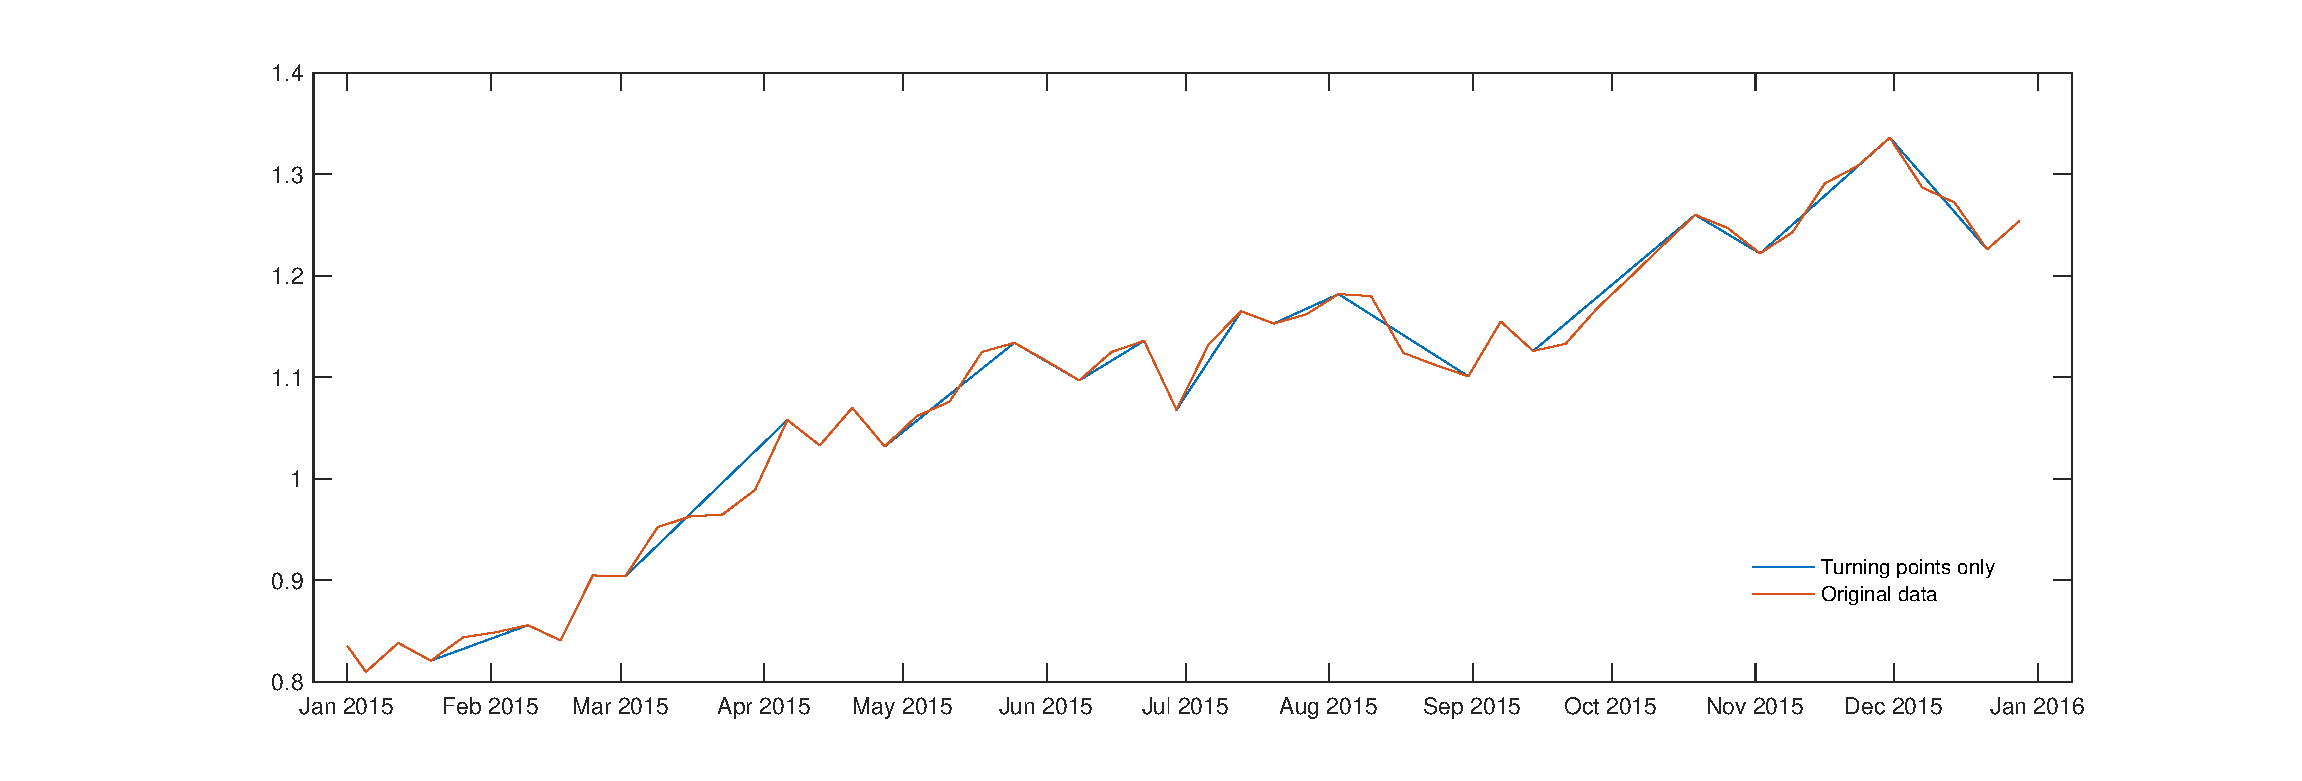
\includegraphics[trim = {0 1.5cm 0 1.5cm}, clip,width=1.8\textwidth]{img/a2a_W_15}}
	
	\caption{\texttt{A2A.MI} weekly 2015. Original data is in the correct position. The other two series are shifted down by 0.1 each.}\label{fig:a2a_w_2015}

\end{figure}




\subsection{Turning points in Python}\label{sec:tp_python}

Python is an excellent language for working with financial data. There is a strong support for downloading, manipulating, and visualising financial market data through popular open source libraries like \texttt{Pandas} and \texttt{Matplotlib}.

In particular, through \texttt{Pandas} we can automatically download data from a number of sources: \begin{itemize}
	\item Yahoo!\ Finance;
	\item Google Finance;
	\item St.Louis FED (FRED);
	\item Kenneth French's data library;
	\item World Bank;
	\item Google Analytics.
\end{itemize}

Focusing on Yahoo!\ Finance, which is our reference source, the set of available indicators is as follows: \begin{itemize}
	\item \texttt{Open};
	\item \texttt{High};
	\item \texttt{Low};
	\item \texttt{Close};
	\item \texttt{Volume};
	\item \texttt{Adj.\ Close}.
\end{itemize}

Let us now go to the code, which is presented in \cref{lst:python,lst:python2} for convenience. The program takes in input the period of time to be considered, the name of the share and the level of deepness. The program is structured in four phases: \begin{enumerate}
	\item prepare, cleaning and convert the data in the time series;
	\item find the local maximum and minimum points (often called \emph{turning points} since they indicate the change in the trend of the stock during a period);
	\item flatten the time serie at different level of deepness;
	\item plot the results.
\end{enumerate}

Actually, we are presenting a slightly different algorithm from the one in our reference paper. When looking for local maximum and minimum points, the conditions \emph{greater}/\emph{less} than were replaced with \emph{greater than or equal to}/\emph{less than or equal to}, and the points at the same level have been adjusted afterwards. This modification brought to a better alignment between the original data and the trend function. The results of some processing are shown in \cref{fig:python}.

\clearpage % TODO Clearpage



\begin{listing}%[H]
 
\inputminted[firstline = 2, lastline = 47]{python}{../code/TPs_Python.py}

\caption{Python implementation (1).}\label{lst:python}

\end{listing}
 
\clearpage % TODO Clearpage

 
\begin{listing}[H]
 
\inputminted[firstline = 50, lastline = 90, breaklines = true]{python}{../code/TPs_Python.py}

\caption{Python implementation (2).}\label{lst:python2}

\end{listing}
 
\clearpage % TODO Clearpage


\begin{figure}%[H]
	
	\makebox[\textwidth][c]{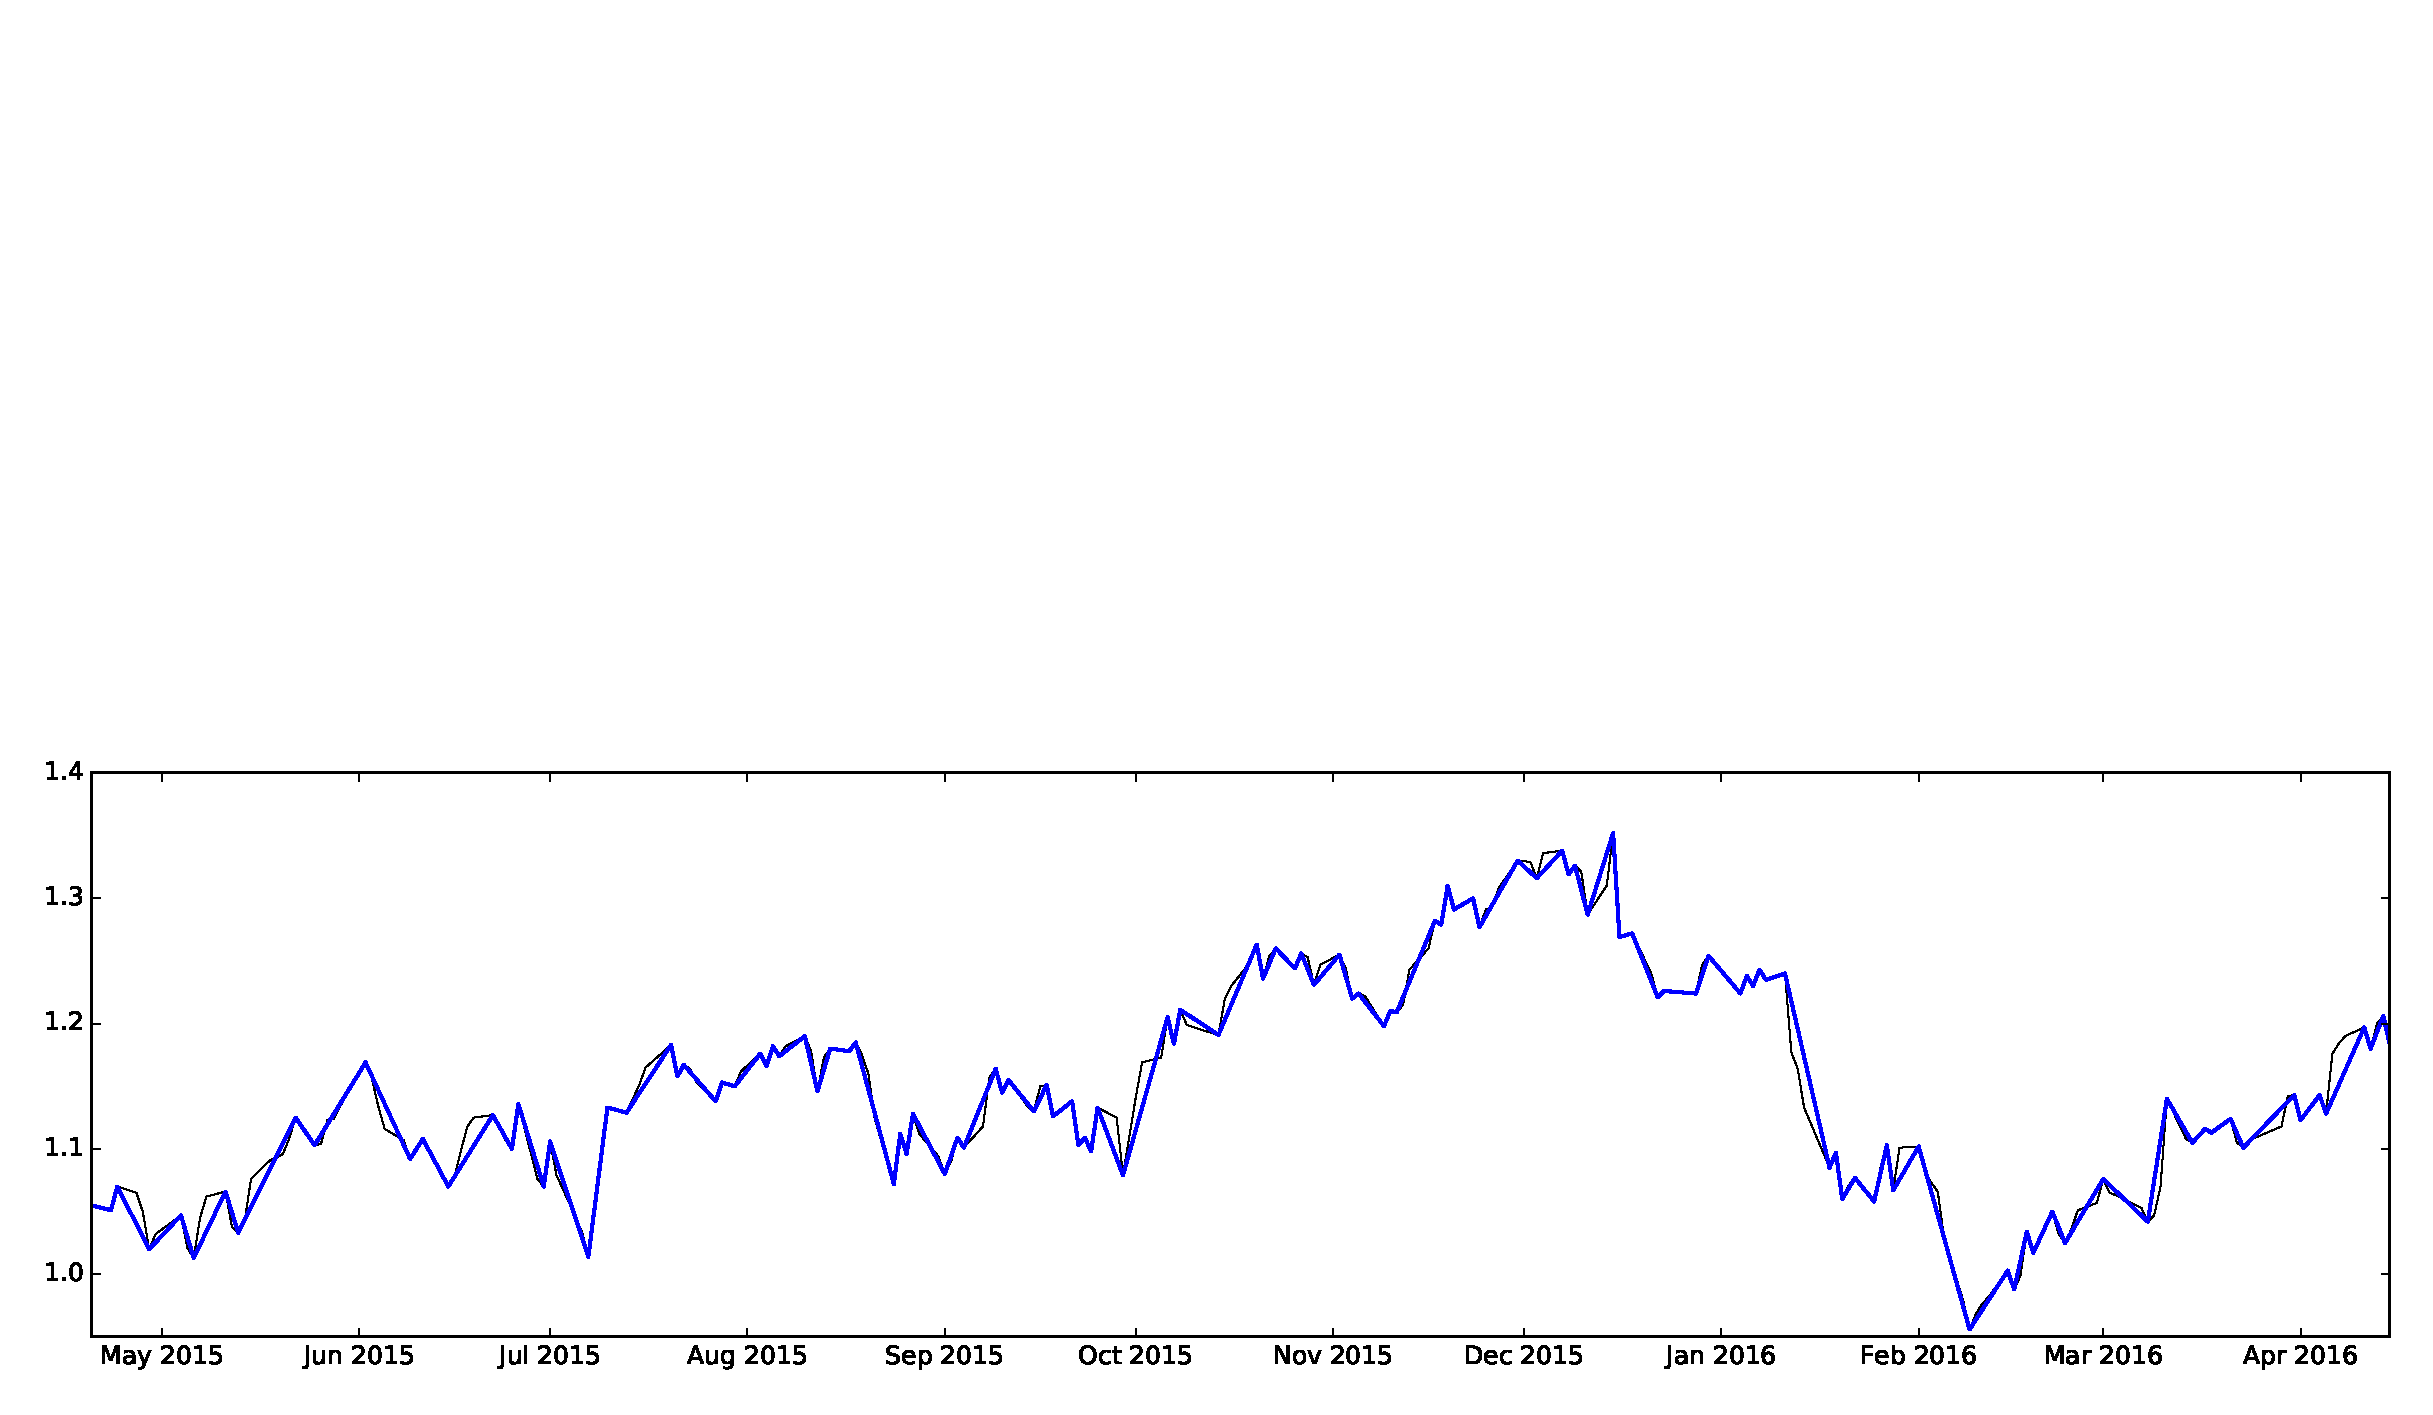
\includegraphics[trim = {0 0 0 12.3cm}, clip,  width=1.5\textwidth]{img/LTP}}
	
	\makebox[\textwidth][c]{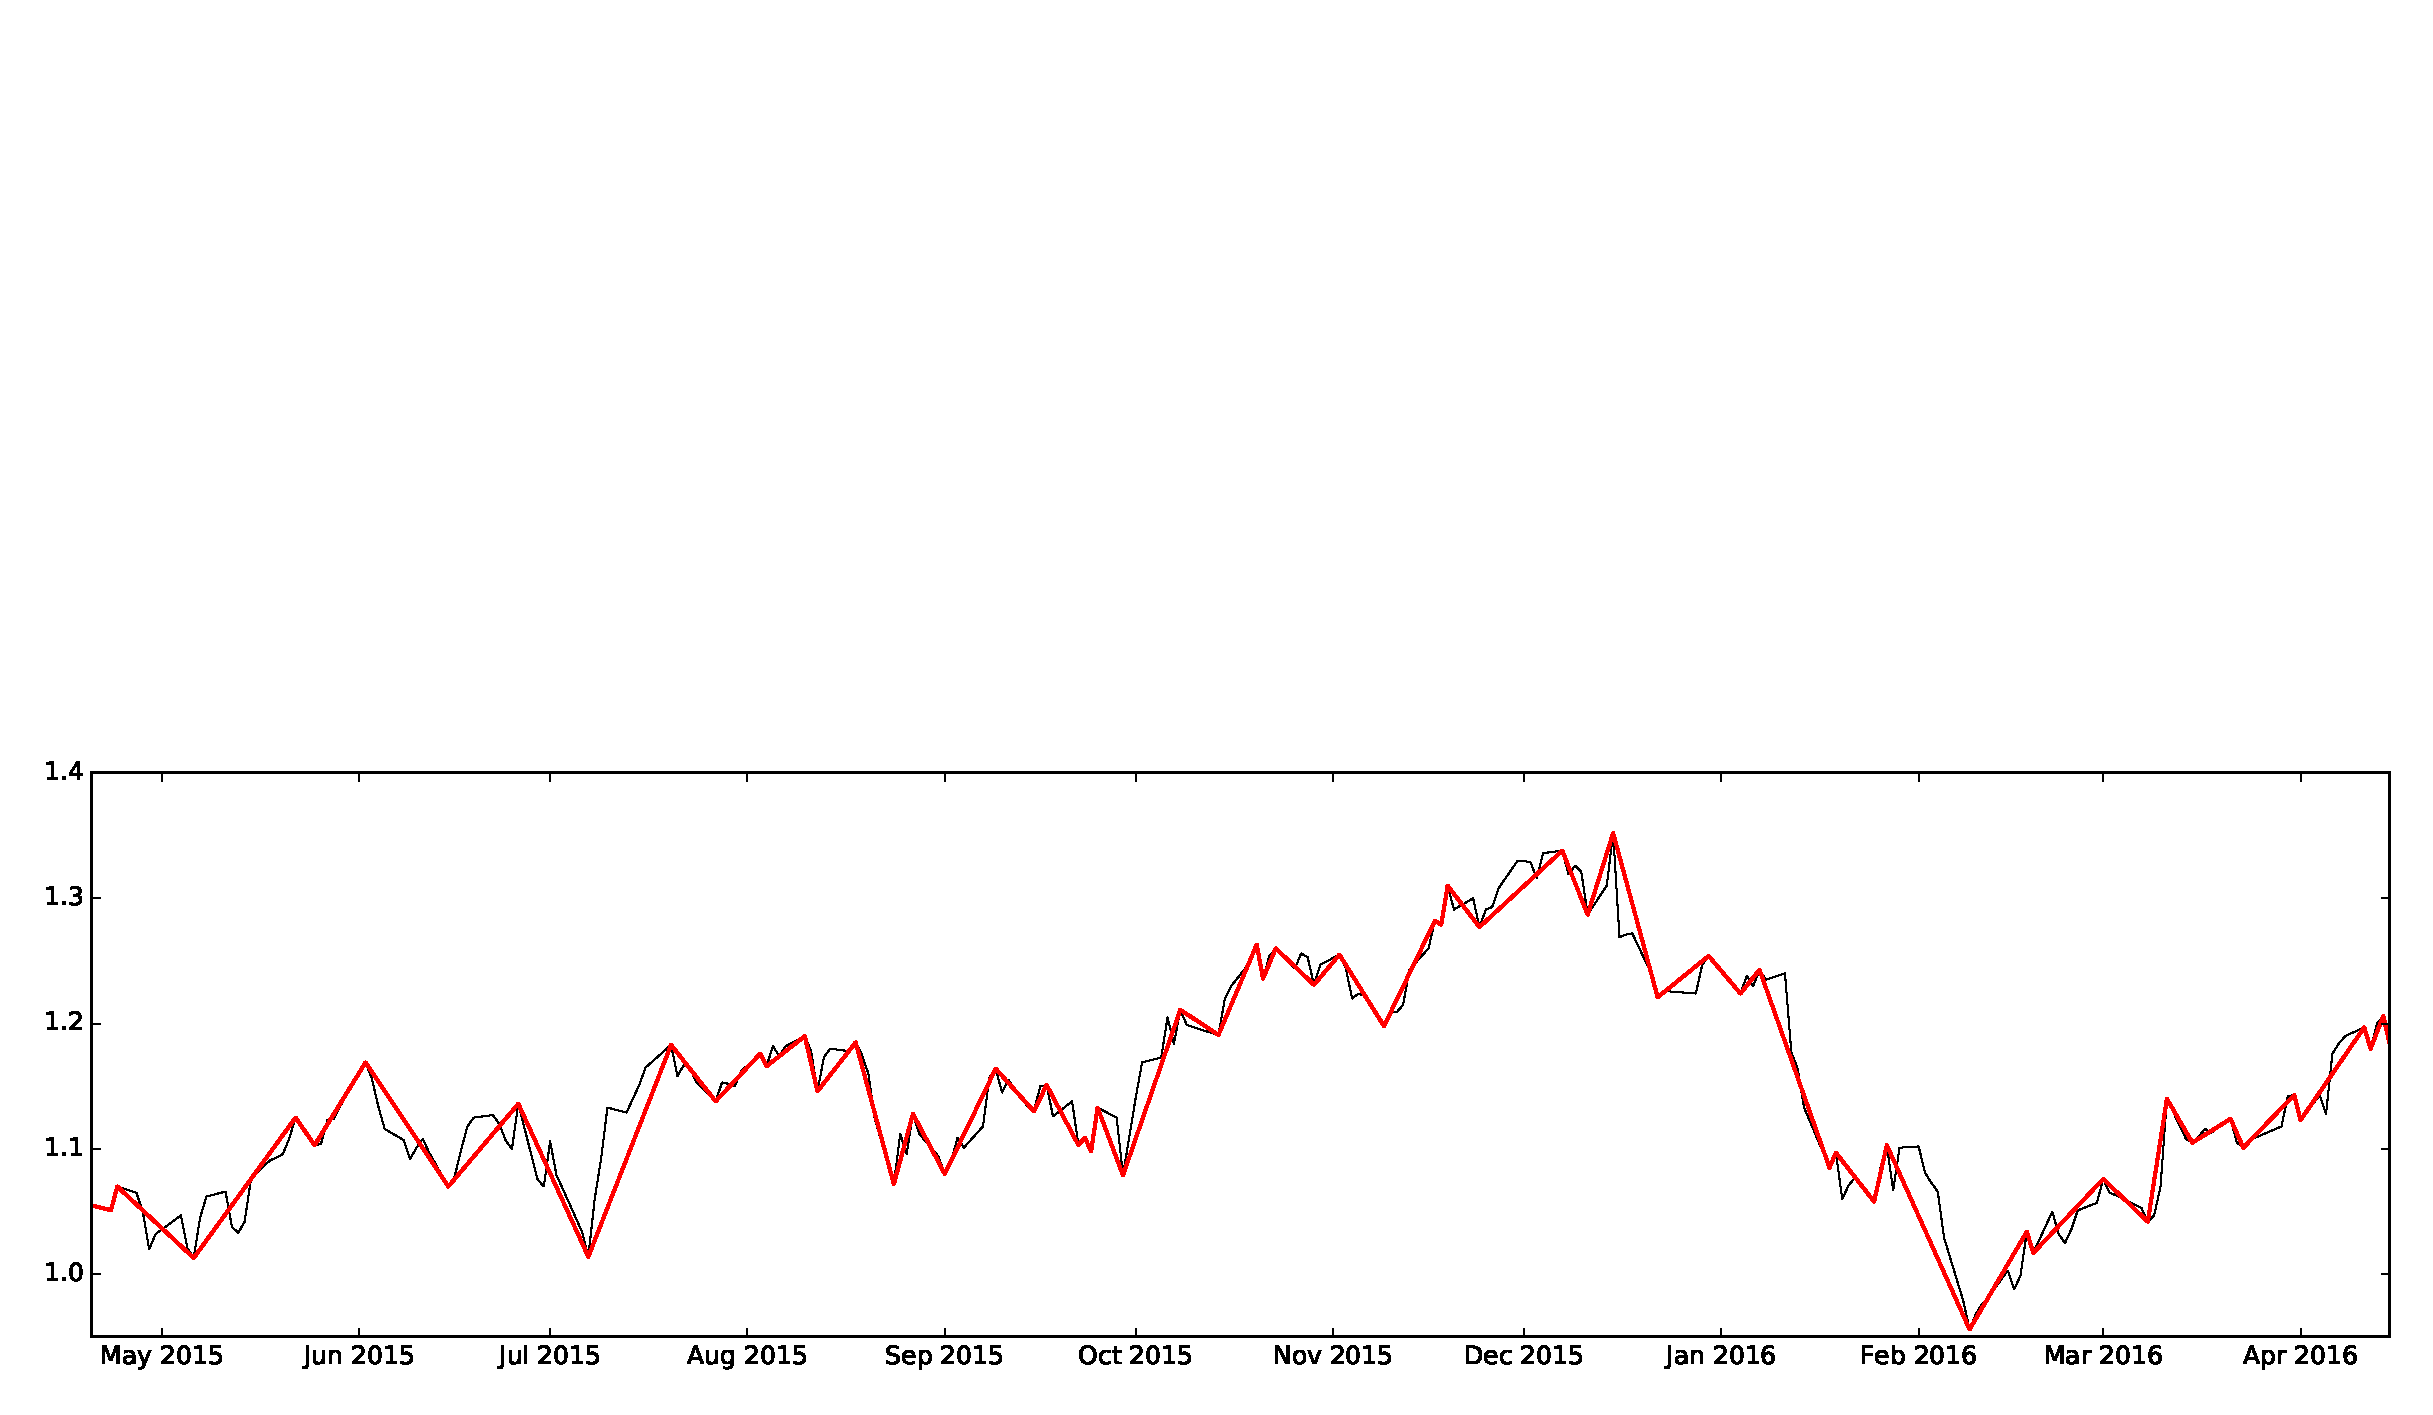
\includegraphics[trim = {0 0 0 12.3cm}, clip,  width=1.5\textwidth]{img/L1}}
	
	\makebox[\textwidth][c]{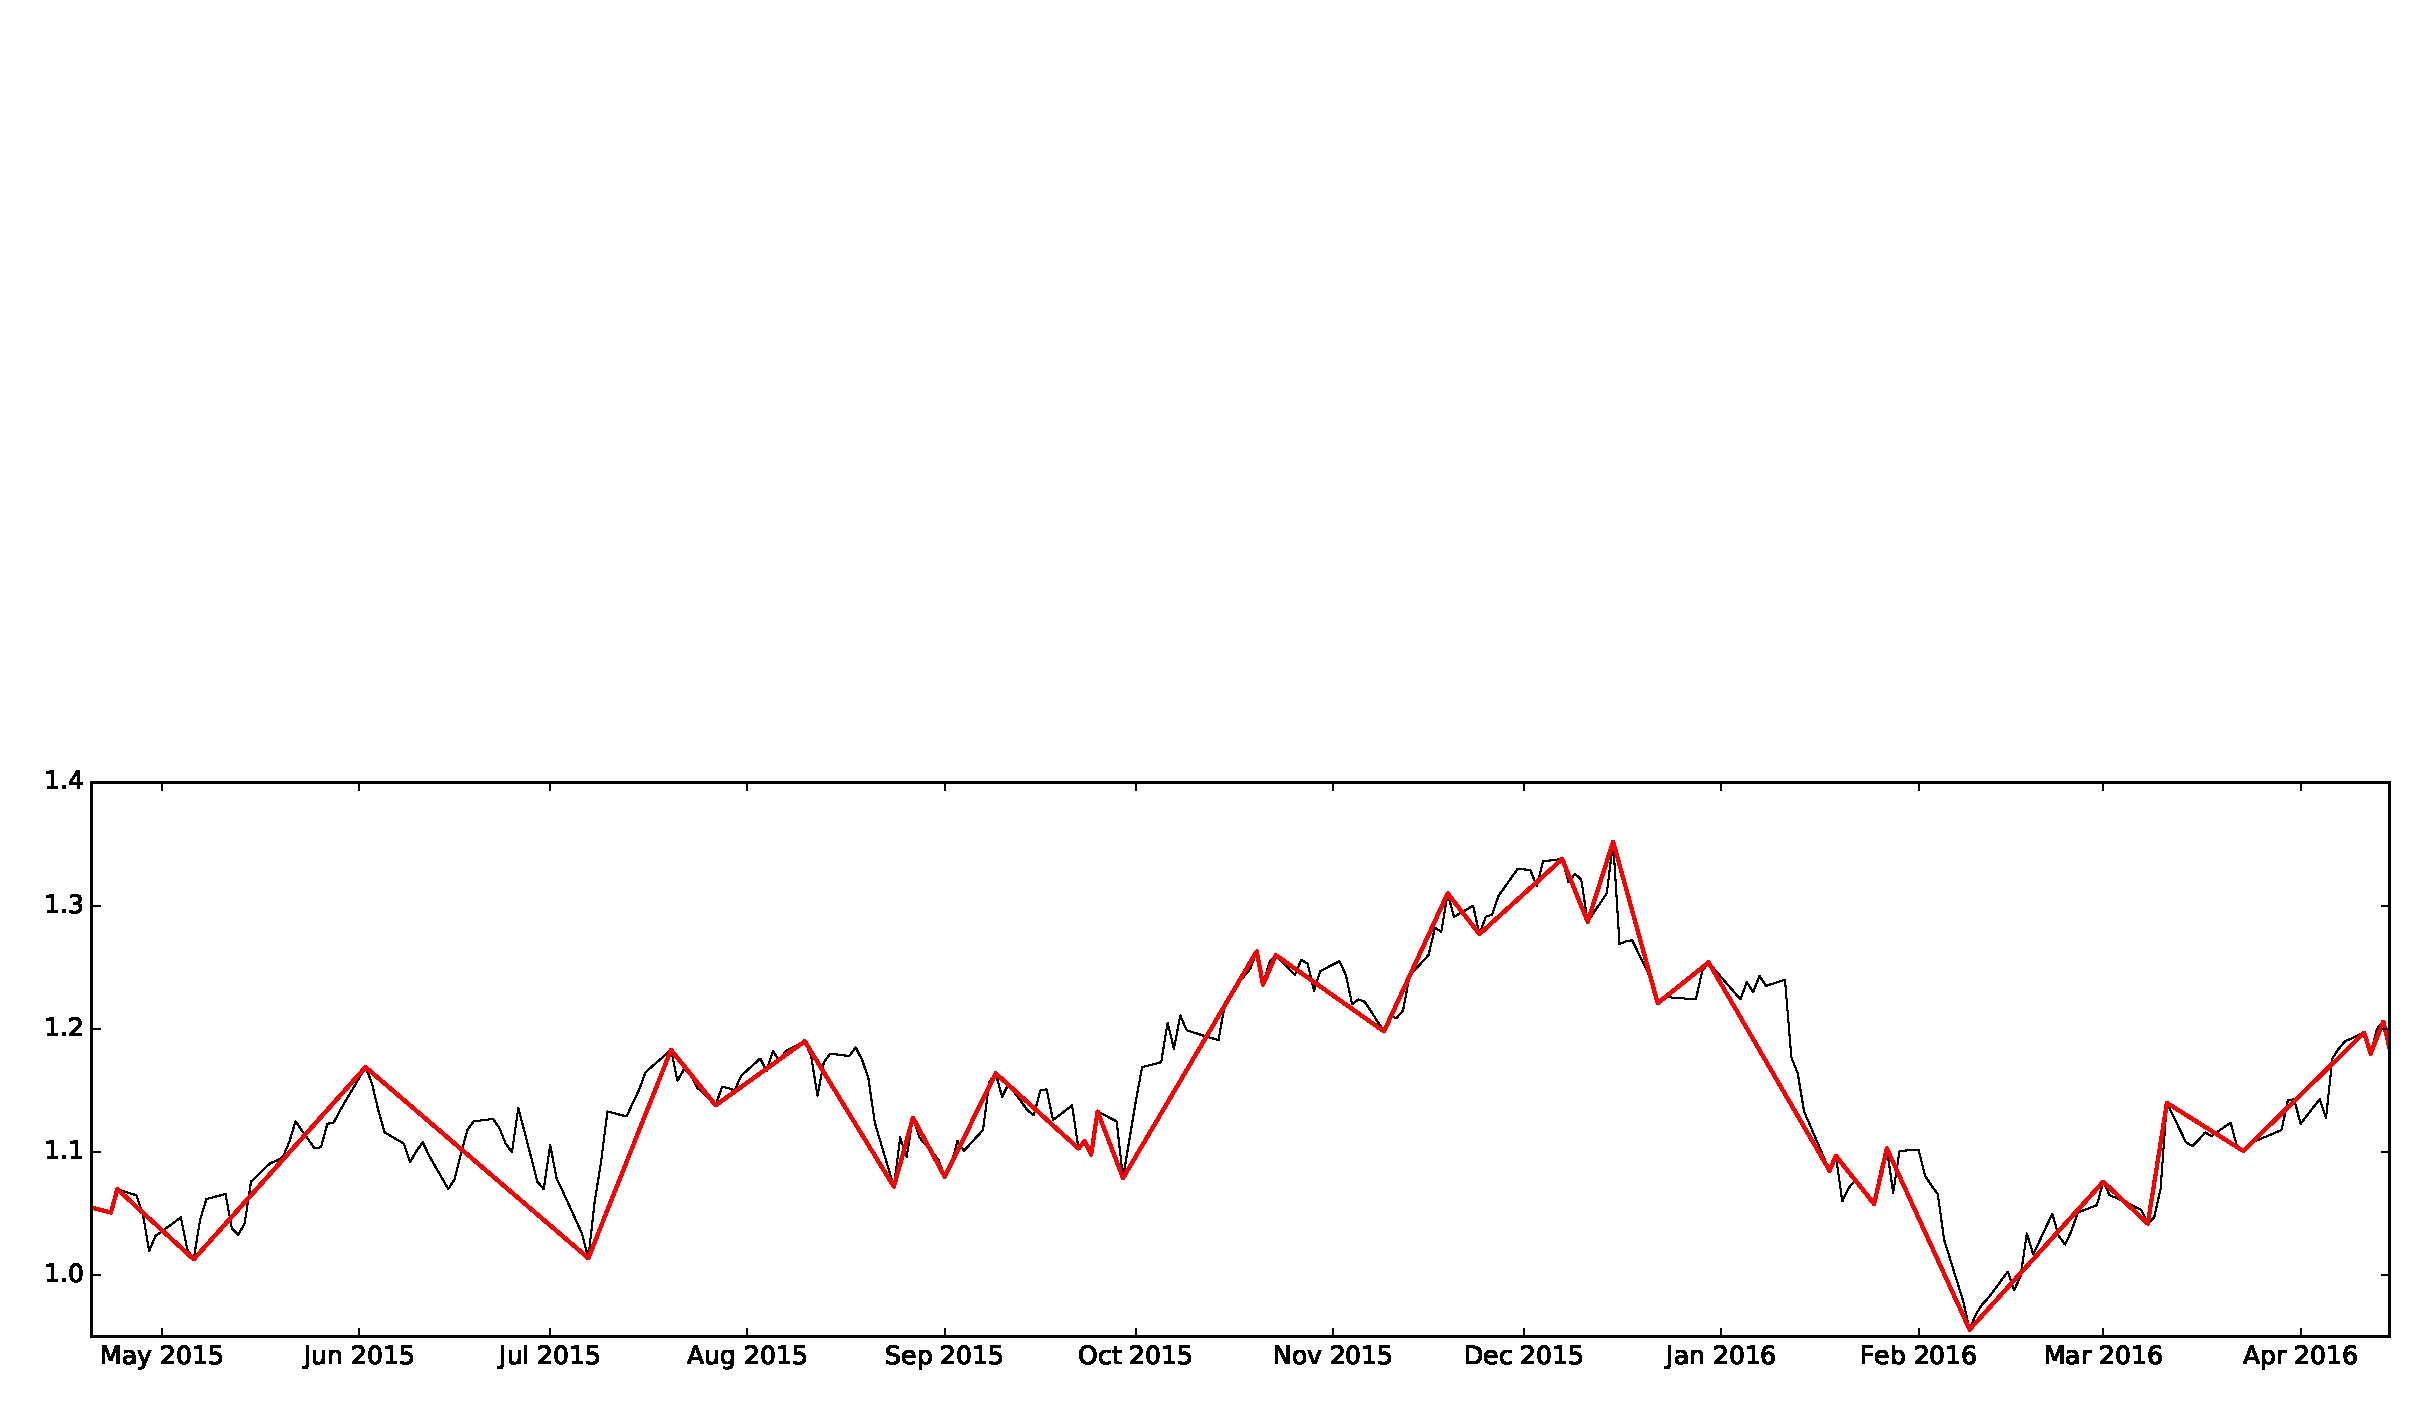
\includegraphics[trim = {0 0 0 12.3cm}, clip,  width=1.5\textwidth]{img/L2}}
	
	\makebox[\textwidth][c]{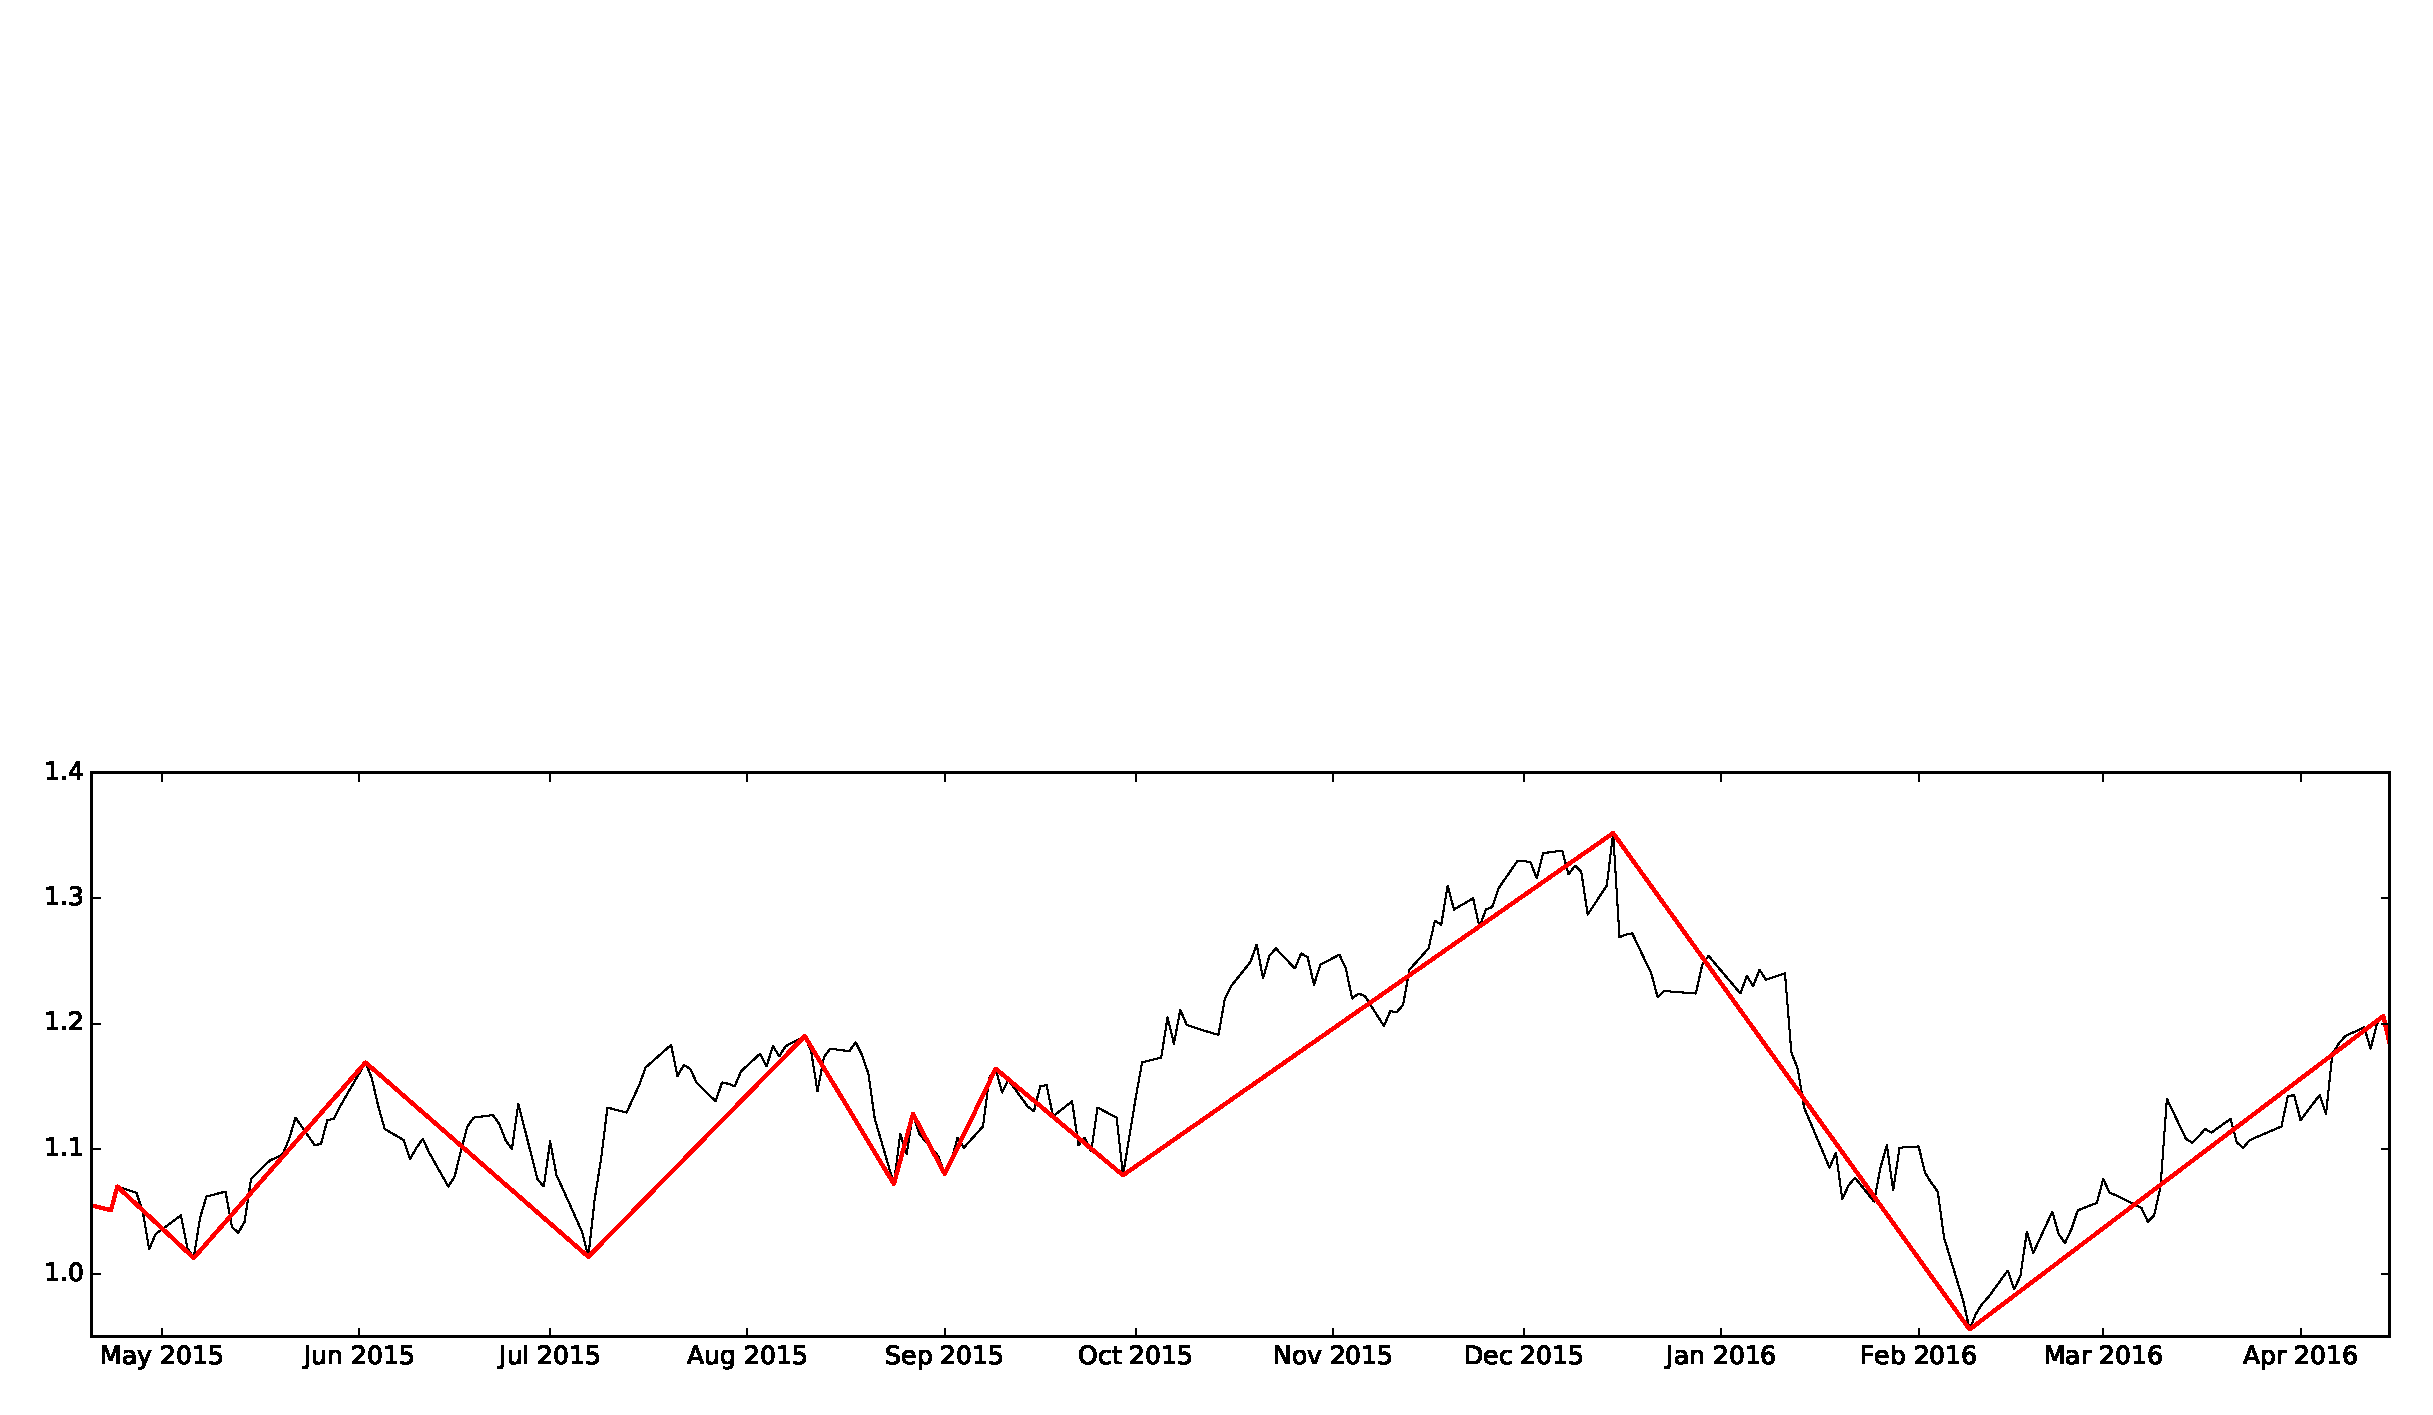
\includegraphics[trim = {0 0 0 12.3cm}, clip,  width=1.5\textwidth]{img/L5}}
	
	\caption{\texttt{A2A.MI} daily \texttt{Close} quotations from mid-april 2015 to mid-april 2016 after preprocessing (local maxima/minima), then after one, two and five iterations of the algorithm.}\label{fig:python}

\end{figure}


\clearpage % TODO Clearpage


\subsection{Other implementations}\label{sec:other}

During our research, we also found an algorithm, developed in the 1970s, named after its three creators: Urs Ramer, David Douglas and Thomas Peucker\footnote{\url{https://en.wikipedia.org/wiki/Ramer-Douglas-Peucker_algorithm}}. We are presenting it rather informally, since it was initially developed for cartographic generalisation, and is now used for the processing of vector graphics.

However, an implementation of the algorithm is already available in \matlab (and others may be easily found in different programming languages), which also gives quite good results (see \cref{fig:rdp}), so we find it appropriate to mention it in this report. 

\begin{figure}[H]
	
	\makebox[\textwidth][c]{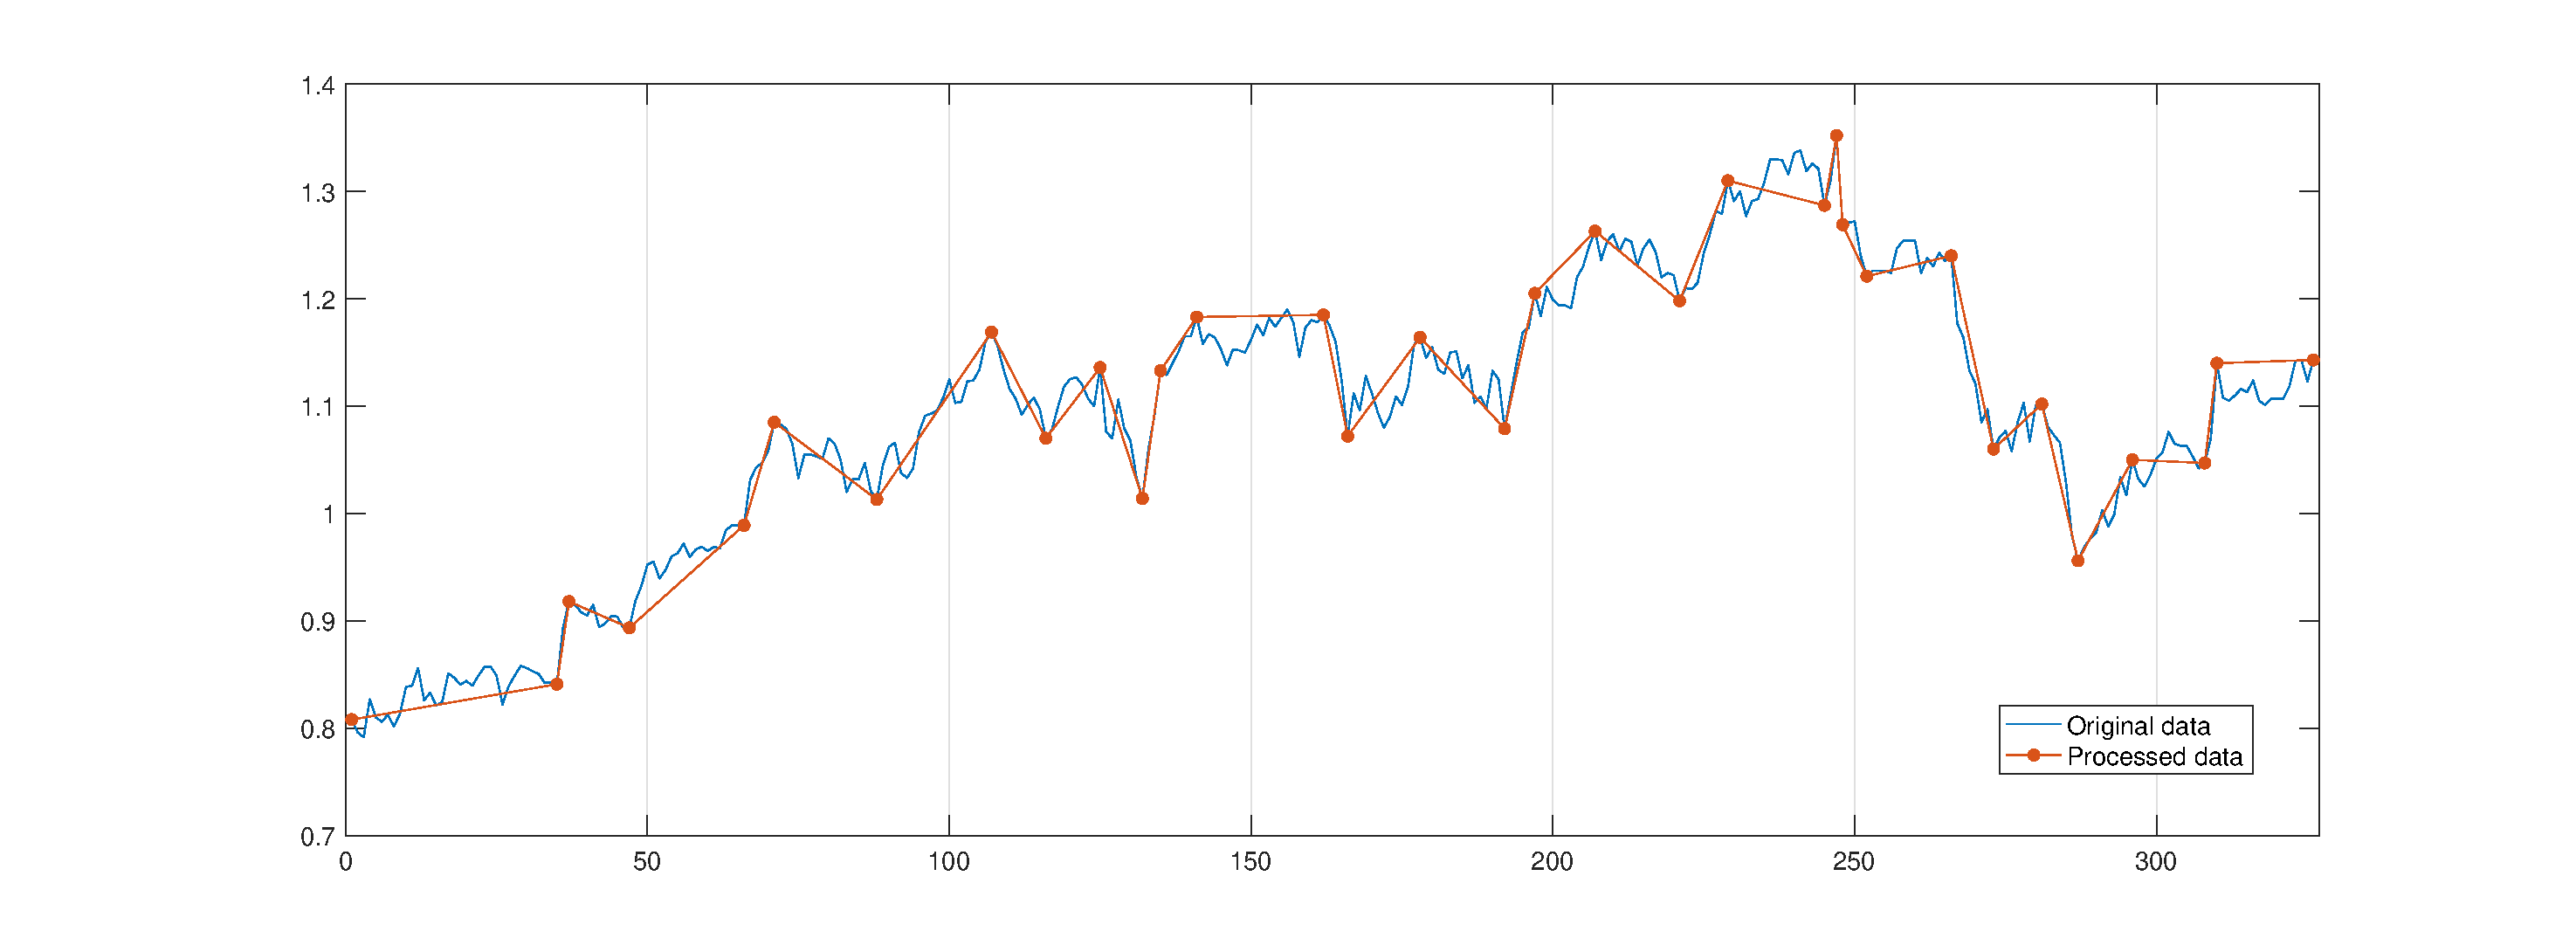
\includegraphics[trim = {0 1cm 0 1cm}, clip,width=1.8\textwidth]{img/rdp}}
	
	\caption{\texttt{A2A.MI} daily stock market data from January 2015 to April 2016.}\label{fig:rdp}

\end{figure}

After installing the add-on\footnote{\url{http://www.mathworks.com/matlabcentral/fileexchange/41986-ramer-douglas-peucker-algorithm-demo}} and importing data, the user may issue the following command: \mint{matlab}{y = DouglasPeucker(M, epsilon, img);}

The results are stored in \texttt{y} matrix. In the command, \texttt{M} is the matrix containing the time series data, \texttt{epsilon} represents the approximation value (in \cref{fig:rdp}, where points range roughly between 0.8 and 1.4, the value 0.05 was used for \texttt{epsilon}), and \texttt{img} is a boolean stating whether the user wants a plot as output (actually, the plot is of really low quality, and the user had better to plot \texttt{y} matrix with standard \matlab commands). 
 
 










\clearpage
\defbibnote{prenote}{DOI (Digital Object Identifier), when defined, serves as URL to retrieve the document. Documents may be accessible only after institutional log in (e.g., academic credentials).}
\printbibliography[title={Bibliography}, prenote=prenote] 




\end{document}







